\pagestyle{headings}

\chapter{Introduction}

\pagenumbering{arabic} 
\setcounter{page}{8}

\section{Motivation}

How much am I paying due to the energy consumption of my fridge? While simple, a typical homeowner do not have access to this kind of information yet. Providing energy usage feedback to homeowners is a helpful way for promoting the energy efficiency \cite{eci}. Detailed information on energy consumption is still invisible to the general population which implies in a source of waste. Without feedback, it is impossible for people to learn effectively about their energy usage patterns, necessary for energy savings. Unlike phone bills in which calls are individually identified, the energy bill shows only the total price which is a limited information. 

As shown in the spectrum of the Fig.~\ref{feedback}, the energy feedback can be either indirect or direct \cite{epri}: 

\begin{itemize}
\item The indirect feedback is provided after the consumption occurs. It may range from a standard electricity bill to daily reports. This is the most common scenario for customers of power utilities nowadays. 
\item The direct feedback is provided in real time with either aggregated or disaggregated energy information. As a difference, aggregated information provides the whole-building consumption information while disaggregated information provides appliance level consumption information.
\end{itemize}


Ideally, users should be able to access disaggregated feedback since more information to the user is provided and thus more control in their decisions. Disaggregated feedback is a valuable resource for homeowners, commercial buildings, and power utilities. For homeowners and commercial buildings, disaggregation helps them making decisions about their consumption habits and appliances to save energy \cite{CarrieArmel2013213}. In addition, it can be helpful to detect malfunctions, inefficient equipment or for scheduling predictive maintenance \cite{eunilm2016}. In regards to power utilities, disaggregation helps them to understand their customers and provide them with better-customized services \cite{eunilm2016-2}. However, the direct feedback might also imply into more costs for implementation, especially if all appliances are connected to a measurement device. In fact, the disaggregation of loads can be accomplished either with intrusion or not intrusively:

\begin{itemize}
\item In an intrusive approach, it is connected one measurement device to each power outlet. This process might lead to high installation costs since it is necessary an infrastructure with one measurement device for each outlet and also a network infrastructure to connect all of them. This solution might also lead to privacy concerns, for example, if the power utility wants to provide an intrusive approach to theirs customers, their employees should go inside all the houses. 
\item On the non-intrusive approach, the energy consumption of the major appliances is estimated using only a single meter installed in the consumer’s energy input panel. The measurements acquired by the energy meter are processed in order to provide details about the operating devices.
\end{itemize}

The advantage of non-intrusive identification is the reduced costs of hardware, maintenance, and privacy. However, non-intrusive identification is still a software challenge due to the complexity of extracting a set of source signals from a mixed signal. This challenge is closely related to the cocktail party problem where there are multiple sound sources recorded by a microphone and we want to extract just one of these sources \cite{ica}. In this context, non-intrusive load monitoring (NILM), also known as load disaggregation, is a research field which seeks to break down a mixed power signal into individual devices.

\begin{figure}[tb]
    \centering
    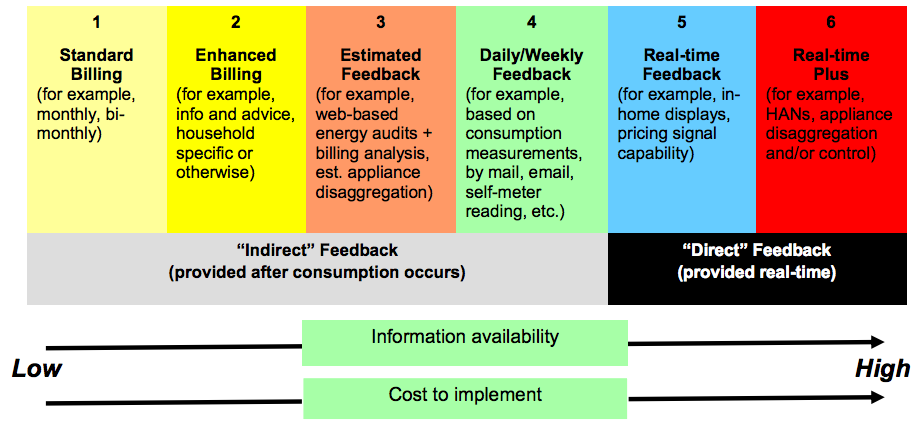
\includegraphics[width=1\columnwidth ]{feedback.png}
    \caption{Spectrum with the different types of energy feedback \cite{epri}}
    \label{feedback}
\end{figure}

\iffalse
How much energy did my fridge spend in the last month? While simple, a typical homeowner still do not have access to this kind of information. The number of energy meters in the world is expected to increase up to 780 Million by 2020 \cite{first}. However, unlike phone bills in which calls are individually identified and marked, the energy bill shows only the total price. No information about the consumption of each appliance is provided. Disaggregation of loads from power measurements is a valuable resource for homeowners, commercial buildings, and power utilities. For homeowners and commercial buildings, disaggregation helps them making decisions about their consumption habits and appliances to save energy \cite{CarrieArmel2013213}. In addition, it can be helpful to detect malfunctions, inefficient equipment or for scheduling predictive maintenance \cite{eunilm2016}. In regards to power utilities, disaggregation helps them to understand their customers and provide them with better-customized services \cite{eunilm2016-2}. The disaggregation of loads can be accomplished either with intrusion or not intrusively. In an intrusive approach, it is necessary to connect one measurement device to each power outlet, which leads to high installation costs and privacy concerns. On the non-intrusive approach, the energy consumption of the major appliances is estimated using only a single meter installed in the consumer's energy input panel. The advantage of non-intrusive identification is the reduced costs of hardware, maintenance, and privacy. In this context, the objective of non-intrusive load monitoring (NILM), also known as load disaggregation, is to break down a whole-home power signal into individual appliances.
\fi

\section{Description of the Problem}

The keyword NILM was introduced in 1985 by George W. Hart in a technical report \cite{hart85} and later published in 1992 by the same author \cite{hart}. \footnote{Nowadays, this keyword have also extended to equivalents NIALM (non-intrusive appliance load monitoring) and NALM (nonintrusive appliance load monitoring). Another commonly and equivalent keyword is load disaggregation.} The paper proposes a full methodology, from types of loads, load signatures, algorithm and physical implementation. The algorithm is based on pattern recognition. Events (edges) are detected and then they are grouped into clusters of active and reactive power. 

However, before introducing the pattern recognition method, Hart describes the NILM problem as a combinatorial optimization (CO) problem. In the CO formulation, the disaggregation is obtained by combining the multiple possible states that minimizes the full measurement for each time instant. For each time instant, we seek to minimize the error between combination of power states and the aggregated measurement. Here, it is assumed that all the possible operating states are previously known. More details about this formulation is presented in the Section 2.2. Hart points three main issues to discourage the usage of this formulation: 
\begin{itemize}
\item The problem has a high computational cost and it increases with the addition of more states of devices or measurements.
\item \textbf{Fundamental Problem}: The complete set of operating states are never known. If the model is used in the presence of unknown appliances, it would attempt to describe their behavior as a combination of other known appliances. 
\item \textbf{Multiple Switching (MS)}: A small change in the measurement might be translated into a big change of the combination of loads. 
\end{itemize}
As shown in the next section, despite various NILM approaches proposed in the literature, very few have attempted in dealing with the CO formulation. While those difficulties are still challenging, there is still room and potential for expanding the formulation in ways to handle the previous problems. This work is especially concerned in solving the MS problem and decreasing their running time of the algorithm. The fundamental problem may also be handled with preprocessing techniques, as shown in the Section 4.  


\section{Previous work}

Figure \ref{1npub} shows the number of publications in the NILM field per year over the last 25 years. Those NILM publications are inferred using publications citing the first NILM work published by Hart in 1992\footnote{Based on \cite{1npub}. Data acquired from Google Scholar. Code available in \url{https://github.com/WittmannF/nilm-publications}}. An exponential growth of NILM publications can be observed since 2010.

\begin{figure}[bt]
    \centering
    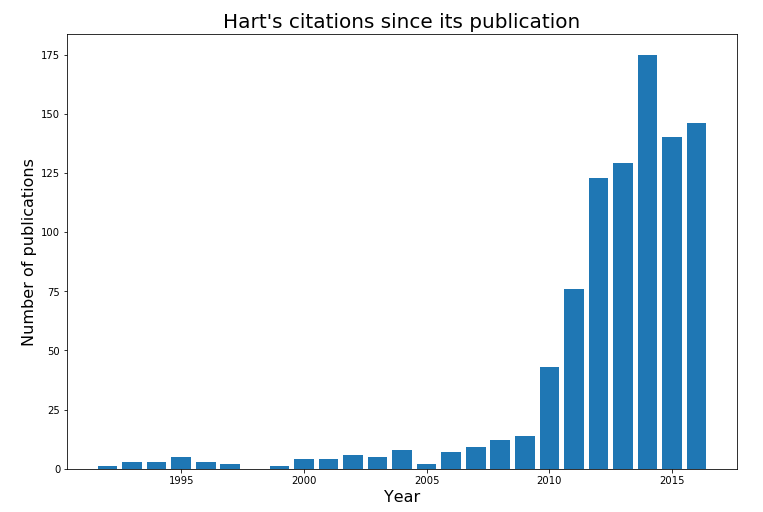
\includegraphics[width=0.8\textwidth]{npub}
    \caption{Number of publications with reference to Hart's original work since its publication}
    \label{1npub}
\end{figure}


%The second problem led the author to propose the switch continuity principle (SCP), which states: \textit{``In a small time interval, we expect only a small number of appliances to change state in a typical load''}. However, as shown in recent works \cite{makonin2016}, SCP is not always reliable. Hence, a better strategy to deal with MS is necessary.
A further analysis in the publication's titles since 2010 did not reveal any trending strategy. Figure \ref{wordle} shows the most frequent words that were found in those titles. Some obvious keywords such as 'nonintrusive', 'load', 'monitoring', 'energy' and 'disaggregation' were removed. As main insights, the NILM research field seems to be mainly focused in residential applications and buildings. Therefore, few attention has been paid to industrial applications. In addition, it seems that privacy is increasingly a concern in the field. Another analysis using only the split of the title after the keyword 'based on' and 'using' was also considered. However, this analysis did not reveal too much insight of key techniques as well. 

\begin{figure}[bt]
    \centering
    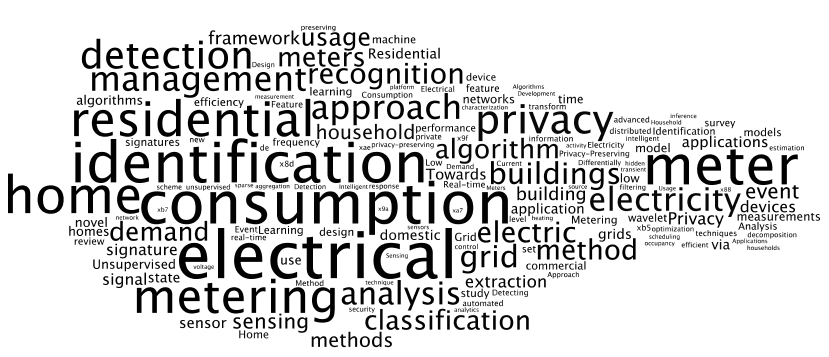
\includegraphics[width=0.8\textwidth]{wordle}
    \caption{Trending words in the titles of NILM publications since 2010}
    \label{wordle}
\end{figure}

There are many ways of categorizing the NILM approaches. For example they can be categorized into either supervised or unsupervised approaches. As defined by Makonin in \cite{makonin2016}, supervised NILM uses measurements of each single appliance to build their models and then disaggregate. Unsupervised NILM does not require single measurements of each appliance for training and allows general appliance models as input which are then tuned to each specific house. Zeifman and Roth in \cite{zeifman} divide the types of algorithms in two categories: pattern recognition (one-to-one matching) and optimization (multiple matching). Nowadays, Zeifman's categorization can be expanded into either event-based algorithms or eventless algorithms. 

The event-based  matching  is  based  on  the  detection  and  classification  of  events. Since the pattern recognition strategies are based on one-to-one matching, the efforts of these strategies are mainly focused on feature extraction. These events are then classified by well-established classifiers, such as k-nearest neighbor \cite{Figueiredo2011}, \cite{berges2009, Froehlich2010}, fuzzy sets \cite{lin2011, ducange2014}, decision trees \cite{Nguyen2015, gillis2016}, support vector machines \cite{duarte2012, zoha2012}, neural networks \cite{zhou2016, bian2016} and deep learning \cite{mauch2016, jack2015}. As noted by \cite{zeifman}, the advantages of pattern recognition methods are that they provide better results in the presence of unknown loads. However, those methods are sensible to the detection of false edges coming from noise or non-linear loads.

On the other hand, eventless methods are based on the simultaneous matching of multiple loads, and they find the set of energized appliances that best fit the measured load. Most efforts from researchers on this side are given methods based on probabilistic models such as hidden Markov models (HMM) \cite{afhmm, reed, hmm_unsup, stephen_hmm}. Other approaches includes sparse coding \cite{sparse_kolter, nmf}, genetic algorithms \cite{meta} and integer programming \cite{suzuki, bhotto2016}. These methods provide better disaggregation performance \cite{zeifman} and are less sensible to edge detection. However, they are more susceptible to the fundamental problem presented in the previous section. 

Regarding the programming approaches, very few of them were focused on expanding the classical CO model. Some of these works are going to be discussed in the next subsection.  

\subsection{Optimization Related Work}

% Egarter and Elmenreich in \cite{meta} verify the MS problem by evaluating six meta-heuristics to solve the CO problem formulated as a knapsack problem. 
\cite{meta} shows the CO pointed in Hart's paper and discusses their equivalency with the knapsack problem. In short, it states that the classic equation is equivalent to the knapsack problem presented in \ref{knap} with a profit $d$ of 1 for all loads, and considering the capacity $C$ corresponds to the total load $P(t)$. However their paper is focused on verifying Hart’s statement regarding the MS. 5 metaheuristics optimization approaches are tested. Their work does not expand the the appliance model, such as new constraints to enhance the identification accuracy. They conclude that it is hard to disaggregate loads with similar power drawns and proposes as future work a multi-objective optimization approach.

\begin{equation} \label{knap}
   max \quad \sum_{i=1}^{n} d_i \ x_i
\end{equation}

$$ s. \ t. \quad \sum_{i=1}^{n} w_i \ x_i \leq C $$

Kolter and Jaakkola in \cite{afhmm} formulate the NILM problem as a convex quadratic programming problem. The authors consider an extension to HMMs, called additive factorial hidden Markov models. Furthermore, authors in \cite{afhmm} describe an unsupervised learning procedure. However, the method needs a regularization parameter that changes for each problem. In addition, the optimization function is made over the full set of time periods, which make the method computationally expensive.

\cite{suzuki} formulates the NILM problem as an integer quadratic programming problem. The technique represents the problem, as a combination of sums of the current of multiple loads. 
At any given one period of current, the overall load current is represented as a superposition of each current of the operating appliance. This is true since the overall current waveform is highly influenced by the waveform of each individual appliance. Each of them has their own properties as shown in the example of Figure \ref{1suzuki}. As advantage, the model considers cases with multiple modes and also same-type operating simultaneously. As limitation, it requires very high frequency data. The model is based on the reading of one cycle (60Hz or 50Hz), so a large number of points from each cycle is necessary.


\begin{figure}
    \centering
    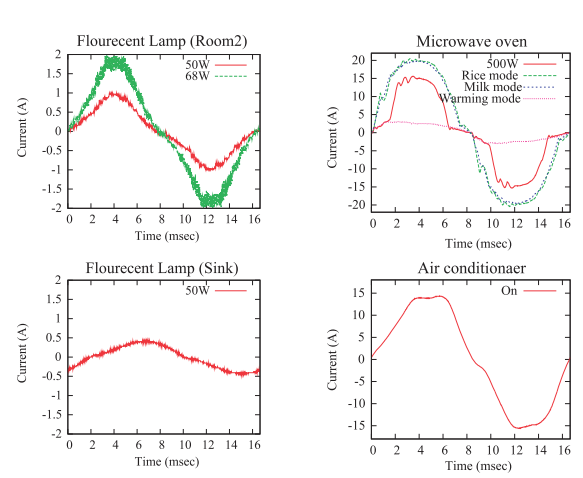
\includegraphics[width=0.8\textwidth]{1suzuki}
    \caption{Example of current waveforms for different loads, used by \cite{suzuki}}
    \label{1suzuki}
\end{figure}

Finally, authors in \cite{bhotto2016} propose a load disaggregation method based on integer linear programming. The work proposes enhancements to CO, such as state transition diagram and median filtering, to deal with the MS. Most enhancements in \cite{bhotto2016} are included as an intensive preprocessing rather than constraints. In addition, their model relies only on instantaneous load samples. Hence, their model is limited to the usage of constraints that does not depend on time measurements.

\section{Objectives}

Based on the efforts made by previous works, the goal of this work is to represent and solve the NILM problem as a mixed-integer linear programming (MILP) problem. We are especially concerned on expanding the classic CO problem in order to deal with complex load signatures. The CO formulation was not very much explored in previous works and this work seeks to propose new constraints for optimizing the identification of loads. In addition, this work seeks to propose strategies to improve the running time of the problem, which is also one of it main weakness. One of this strategies is to formulated the classic CO problem as a linear problem and propose linear constraints to the model. Another objective of this work is to compare the formulation with classic formulations. Most previous works are based on either event based techniques or probabilistic models and this work allows researcher to expand the range of possibilities and approaches.  in  dealing with the MS problem and compare with other methods based on pattern recognition and CO.

%The contributions of this work are brought from (). The work deals with the unit commitment problem in which try to allocate multiple combination of termal units for a given period. The constraints for modeling time and x demonstrates to be useful for NILM . 

\section{Contributions}

The main contributions of this paper are as follows:

\begin{itemize}
\item The NILM problem is represented as a MILP model, in which a new set of integer linear constraints is proposed to efficiently model the load signatures of the appliances.
\item In order to enhance the computational performance, the proposed NILM is solved using a window-based algorithm in which the overall problem is segmented into small, coupled sub-problems that can be efficiently solved via commercial MILP solvers.
\item The proposed model is also suitable for unsupervised NILM in the context described in \cite{makonin2016}. The model relies in parameters that can be acquired from aggregated data, such as, minimum operation time and sequence of states.
%\item A new set of constraints to model the load signature
%\item A window based algorithm in order to make the algorithm to run more efficiently
%\item The problem that led Hart to propose the \textit{switch continuity principle} is avoided in the tests cases
\end{itemize}

\section{Organization of the Work}

The next sections of this dissertation goes in this way:
\begin{itemize}
\item The Chapter 2 describes some background work that is used as basis for the remaining chapters. The reader may skip subsections that are already familiar with. 
\item The Chapter 3 describes the main contributions of this work. A math model for modeling the load signature. 
\item The Chapter 4 describes the process of extracting the features that are used for feeding the input table of the model. The chapter is divided into two subsections: A supervised approach which uses clustering for extracting the main information and an unsupervised approach which is based on edge detection and histogram analysis.
\item The Chapter 5 describes the test cases with results for both the unsupervised setting and the supervised one. 
\item Finally, the Chapter 6 presents the main conclusions and future work. 
\end{itemize}